% Manuel Lippert - Paul Schwanitz
% Physikalisches Praktikum

% 3.Kapitel  Protokoll

% Variables
\def\skalierung{0.65}

\chapter{Messprotokoll}
\label{chap:protokoll}

Das Messprotokoll wurde am Versuchstag handschriftlich erstellt und hier als
PDF-Datei eingefügt. Dabei wurden Durchführung und Aufbau schon vorher in dieses
Dokument beschrieben, je nachdem.

\section{Versuchsaufbau und Beschreibung}
\label{sec:aufbau}

% Manuel Lippert - Paul Schwanitz
% Physikalisches Praktikum

% 3.Kapitel  Protokoll 

\subsection{Invertiertes Pendel}
\label{sub:aufbauPendel}
% TODO: #24 Aufbau Pendel @ManeLippert

\subsection{Aufgabe Bifurkationsdiagramm}

Messung zu 3.3.1 aus Versuchsanleitung.
Vermessung der Gleichgewichtslage in Abh. der Masse.
Messfehler Waage: 
\begin{align}
    s_a = 0,005\, g \\
    s_r =
\end{align}

Messfehler Multimeter: 
\begin{align}
    s_a = 0,00005
\end{align}
starke Schwankung der letzten Ziffer.
\begin{align}
    s_r =
\end{align}

Länge des Pendels (mit Stahlmaßstab): 
\begin{align}
    l = 37 \, cm
\end{align}

Gewicht Feststellschraube: \(m_s = 3,14 \,g\)

Der Fehler der Auslenkung wird aufrund der Schwingungen während der Messung größer angenommen.\\


Teil 2: Prüfung der Ergebnisse.
Freie Schwingung des Pendels; Auslenkung bis ca. 1V; Messung der Schwingunsdauer (10fach).
Zeitmessung mit Smartphone.\\
Schwingunsdauer.csv; Messung ohne Masse.\\
Schwingunsdauer1.csv; Messung mit 12,58 g.\\

Grobe Auswertung: \(M_k = 19,3 \, g\)

\subsection{Aufgabe: Schwache Nichtlinearität}
\paragraph{Teol a)}
Mantage Dämpfungssegel; Masse Dämfungssegel: \(m=4,4 \, g\)\\
restliche montierte Masse: \( m = 10,42 \,g \)


\paragraph{Teil b)}
Montage Dämfungssegel;\\
Masse Dämfungssegel: \(m=4,4 \, g\)\\
restliche montierte Masse: \( m = 10,42 \,g \)

Messung mit Messprogramm gestartet: 2000 Steps; Start: 0Hz; End: 1,1Hz


\subsection{Aufgabe: Starke Nichtlinearität}
Montage Dämfungssegel;\\
Masse Dämfungssegel: \(m=4,4 \, g\)\\
restliche montierte Masse: \( m = 19,44 \,g \)

\paragraph{a)}
Labview Absturz bei 0,517 Hz 
Neustart 0,52 Hz

quasichotisch ? bei 0,411 Hz

Frequenzen den Daten entnehmen.


\paragraph{b)}

Startbed: \\
Montage Dämfungssegel;\\
Masse Dämfungssegel: \(m=4,4 \, g\)\\
restliche montierte Masse: \( m = 19,44 \,g \)
Anregfreq.: 0,411Hz

Strittmotor in Anfagspos. (ganz unten)


% Manuel Lippert - Paul Schwanitz
% Physikalisches Praktikum

% 3.Kapitel  Protokoll

\subsection{Shinriki-Oszillator}
\label{sub:aufbauShinriki}

\begin{figure}[h]
    \centering
    %TODO #31
    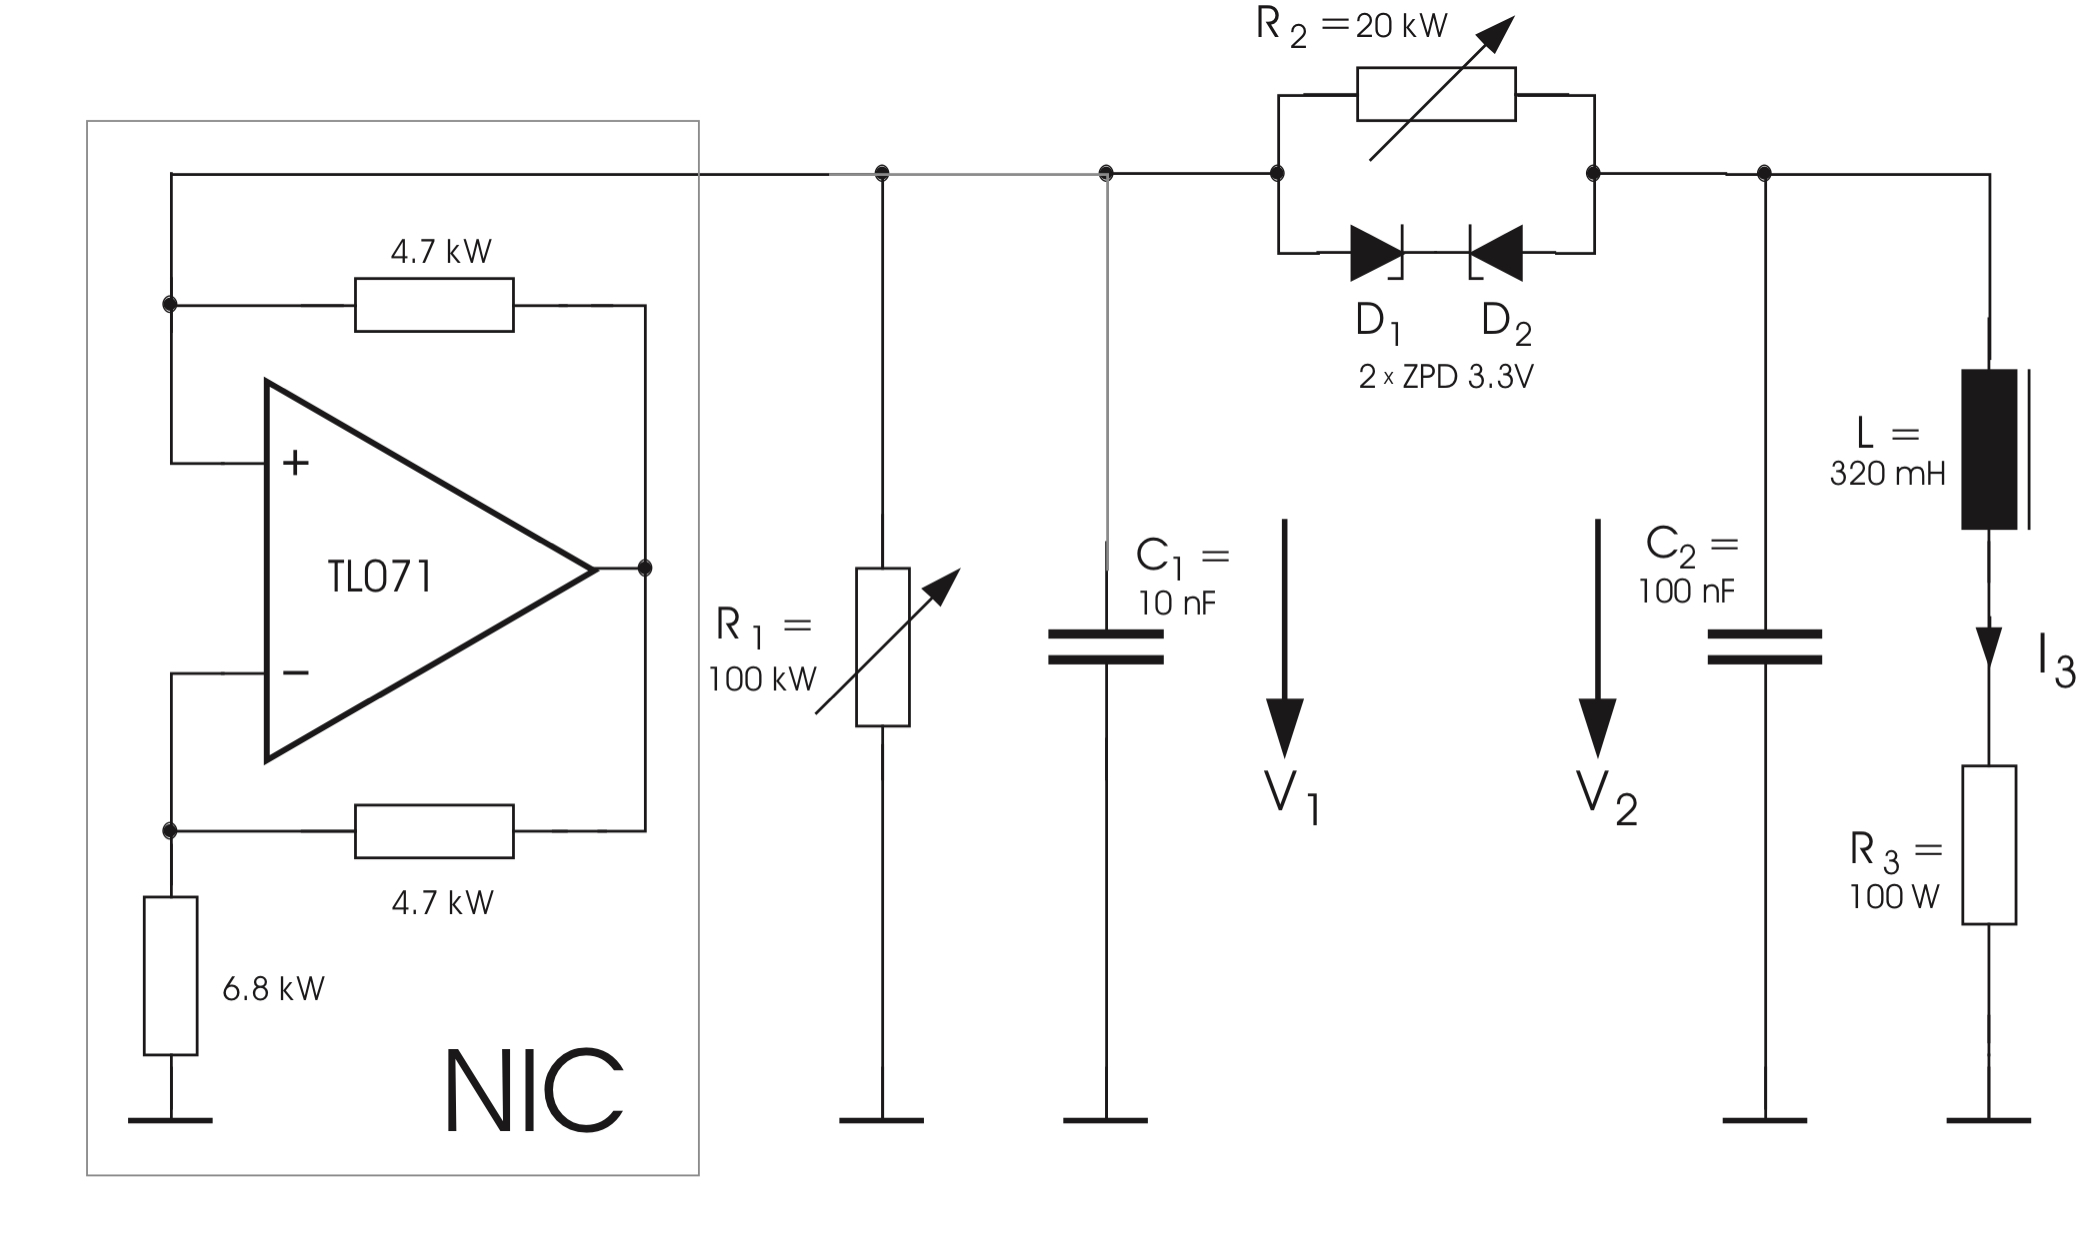
\includegraphics[scale=0.15]{ShinrOsziSp.jpeg}
    \label{fig:shinrikiSp}
    \caption{Schaltplan des Shinriki-Oszilator}
\end{figure}
% TODO: #25 Aufbau Shinriki @PaulSchwanitz

\section{Versuchsdurchführung}
\label{sec:durchfuehrung}

% Einbindung des Protokolls als pdf (mit Seitenzahl etc.)
% Erste Seite mit Überschrift
%\includepdf[pages = 1, landscape = false, nup = 1x1, scale = \skalierung , pagecommand={\thispagestyle{empty}\chapter{Protokoll}}]
%            {03-Protokoll/Protokoll.pdf}
% Restliche Seiten richtig skaliert
%\includepdf[pages = -, landscape = false, nup = 1x1, scale = \skalierung , pagecommand={}]
%            {03-Protokoll/Protokoll.pdf}